%!TEX encoding = IsoLatin

%
% Chapitre "Conceptualisation et analyse de faisabilité"
%

\chapter{Conceptualisation et analyse de faisabilité}
\label{s:conceptualisation_et_analyse}

\section{Diagramme fonctionnel}

\begin{figure}[!htb]
    \centering
    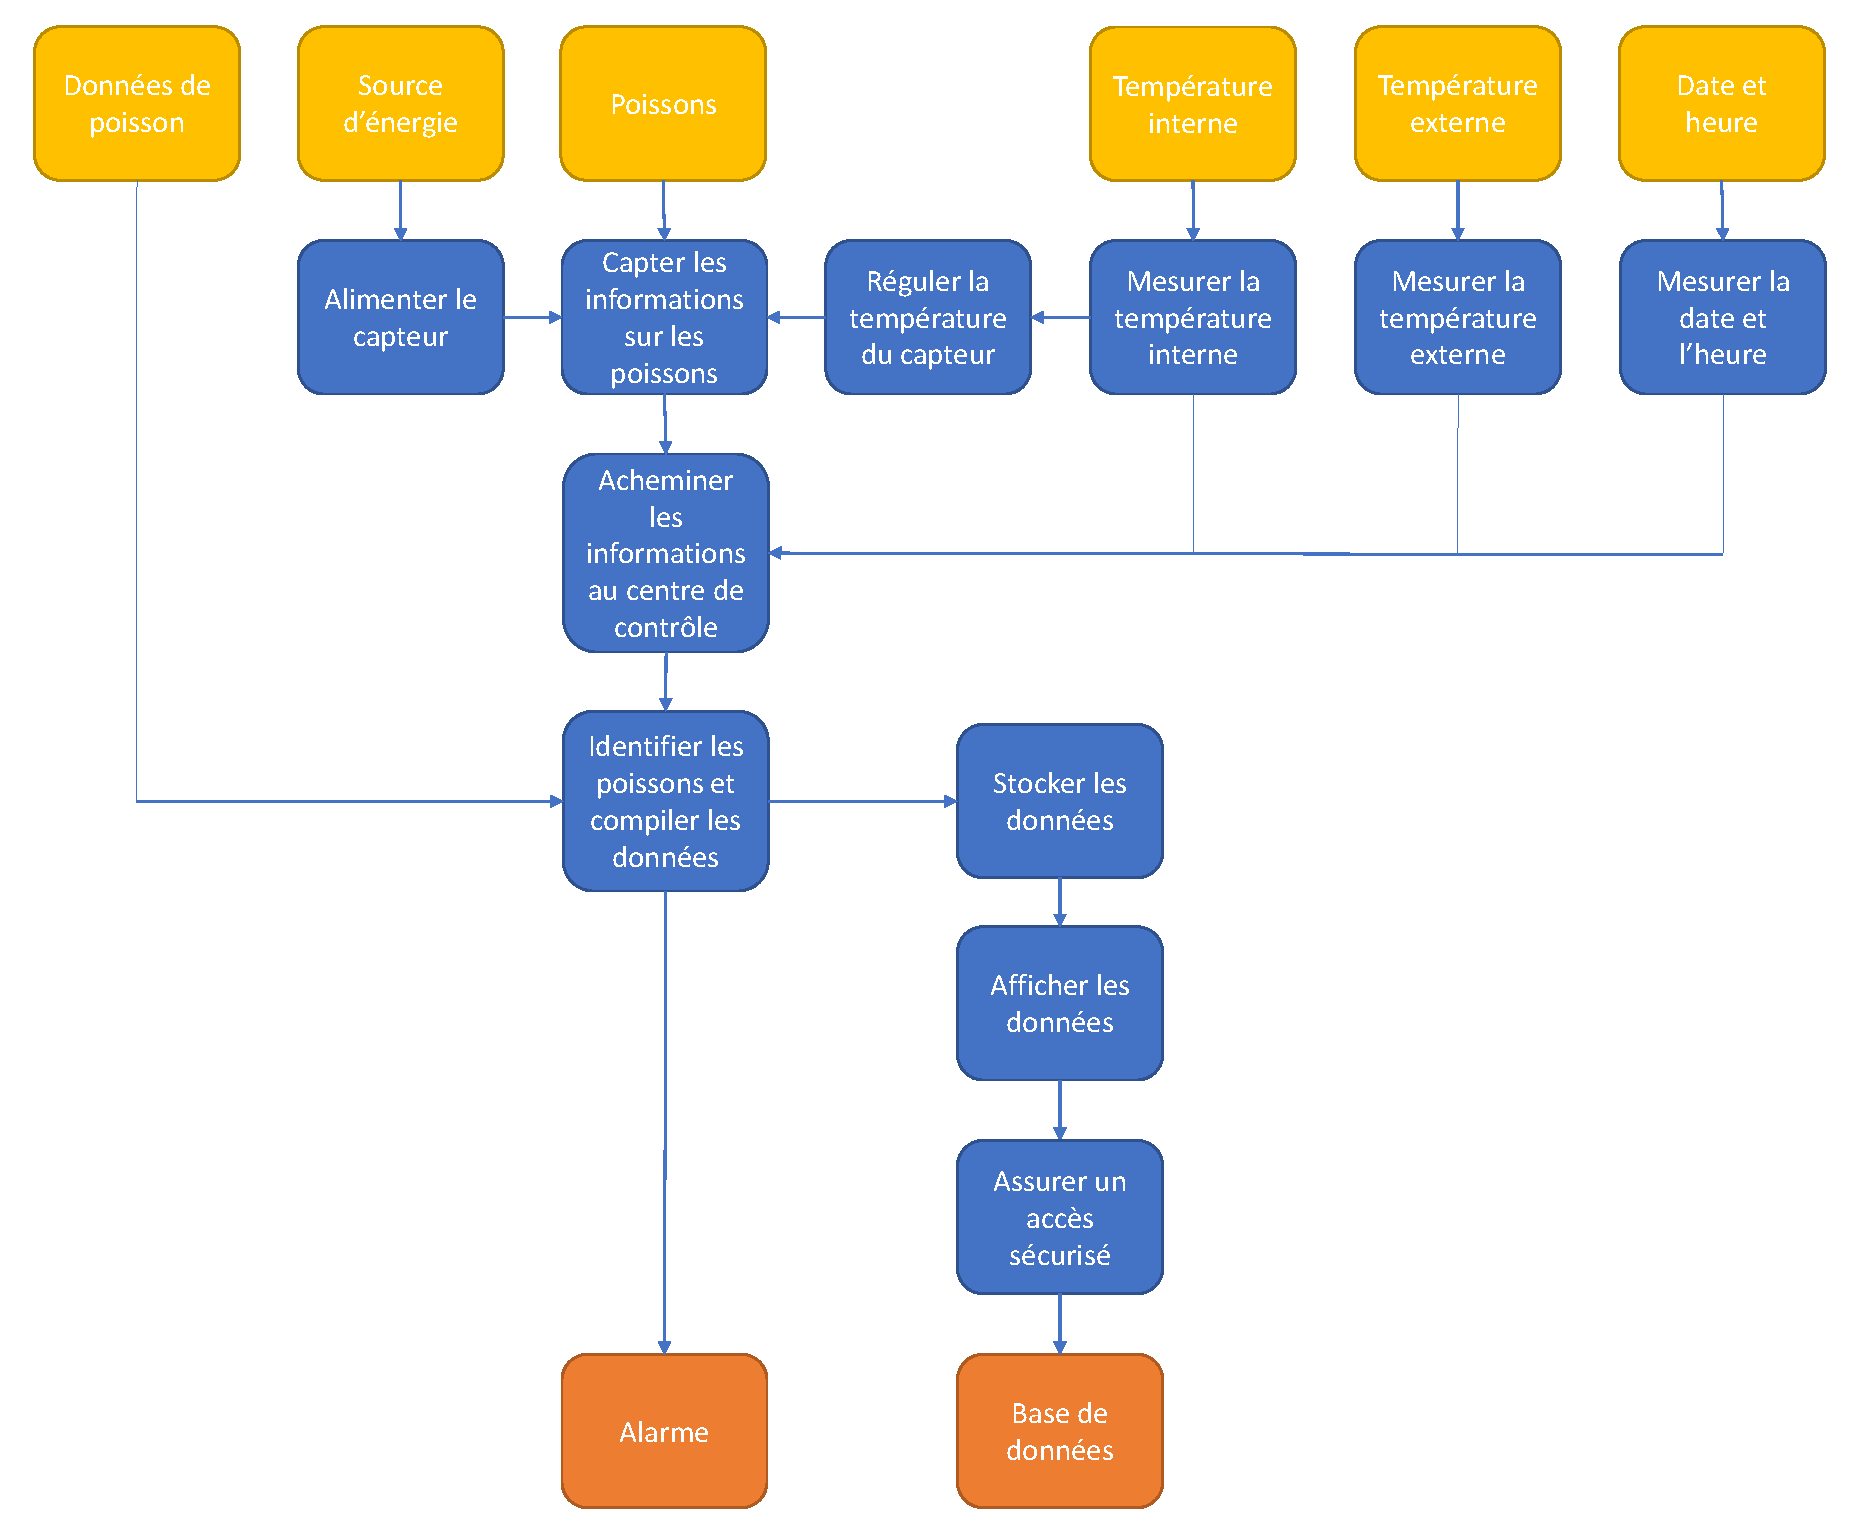
\includegraphics[width=0.80\linewidth]{fig/Diagramme_fonctionnel.pdf}
    \caption{Diagramme fonctionnel du projet Fish \& Chips}
    \label{fig:diagramme_fonctionnel}
\end{figure}

La figure \ref{fig:diagramme_fonctionnel} présente le diagramme fonctionnel du design pour le projet Fish \& Chips. Les intrants y sont présentés en jaune, les fonctions en bleu et les extrants en rouge.

Les intrants constituent toutes les données nécessaires au projet que l'on extrait de l'environnement. Les poissons sont au coeur du projet: à l'aide d'une mesure passive, ils devront être analysés et identifiés par un système de reconnaissance. Le MFA souhaite comptabiliser les espèces de poissons d'eau douce du Québec qui font plus de 6 cm de long. Pour ce faire, des données de poissons seront fournies au système de reconnaissance. Elles seront sous une forme de base de données qui comprendra plusieurs photos de poissons de chaque espèce sous différents angles de vue avec leur espèce correspondante. Cela servira à l'entraînement ou de référence au système d'identification. Ensuite, une source d'énergie sera tirée de l'environnement ou d'une composante pour alimenter le dispositif qui sera chargé de capter les données brutes sur les poissons. La température interne du dispositif de mesure des poissons, la température de l'eau ainsi que la date et l'heure sont nécessaires à la création de la vignette. De plus, certaines de ces données serviront à déterminer s'il y a une erreur dans le système pour avertir un utilisateur.

Les extrants du système sont les choses qui seront produites par le système. Le point central du design est de produire une base de données contenant toutes les vignettes de poissons identifiés, les statistiques sur les populations des différentes espèces, les images originales enregistrées pour une durée de 2 ans ainsi que d'autres informations connexes comme les commentaires, les paramètres de configuration et les alarmes. Les alarmes seront envoyées à un responsable sous la forme d'un message lui avertissant que le fonctionnement du système peut être compromis.

\pagebreak

\section{Conceptualisation et analyse des solutions}

\subsection{Capter les informations sur les poissons}

Afin d'optimiser et de faciliter l'identification des poissons, il est nécessaire d'utiliser un système de détection de qualité. En ce sens, il est primordial que le capteur optique utilisé soit fiable et efficace. Le capteur optique a comme responsabilité de détecter les poissons de même que prendre une image de ceux-ci. Cependant, son utilisation ne doit en aucun cas perturber l'environnement de la faune aquatique. \vspace{5mm}


\textbf{Aspects physiques:}
\begin{itemize}[label = {--}]
    \item Sous l'eau, la solution doit posséder une masse inférieure à 5kg.
    \item Sous l'eau, la solution doit posséder un volume de moins de 0.3m$^3$.
    \item La solution doit être utilisable jusqu'à une profondeur de 50 pieds.
    \item La température interne de la solution doit rester entre -6°C et 30°C.
\end{itemize}

\textbf{Aspects économiques:}
\begin{itemize}[label = {--}]
    \item La solution doit être la moins dispendieuse possible.
\end{itemize}

\textbf{Aspects temporels:}
\begin{itemize}[label = {--}]
    \item Le temps de développement de la solution doit être minimisé.
\end{itemize}

\textbf{Aspects socio-environnementaux:}
\begin{itemize}[label = {--}]
    \item La solution doit assurer une mesure passive.
\end{itemize}

\subsubsection{GoPro Hero7 Black Edition}

\textbf{Description:} La GoPro Hero7 Black comporte plusieurs fonctionnalités. Elle peut prendre des images de 12 méga-pixels à grande gamme dynamique (HDR) et des vidéos allant de 720p à 4K. La GoPro peut également prendre entre 24 et 240 images par secondes. Elle comprend un système de stabilisation d'images idéal pour la détection de poissons et un mode pour la vision nocturne. Sa fonctionnalité « Live Streaming » ainsi que son système de connexion Wi-Fi et Bluetooth intégré permettraient également de relever les données sur les poissons en temps réels. Un système intégré GPS permet de la localisé en tout temps. La GoPro est livrable entre 3 et 6 jours a des frais d'environ 560\$. \vspace{5mm}

\textbf{Décision:} Retenue, mais. \vspace{5mm}

\textbf{Justification:} La GoPro Hero7 Black Edition comporte de nombreux avantages et réponds aux exigences du client. En effet, la masse de la caméra est de 0,116kg et son volume est de 9,2309x10$^{-5}$m$^3$. Il s'agit d'une caméra très fiable et utilisée dans des conditions climatiques extrêmes. Cependant, la GoPro peut seulement atteindre une profondeur de 33 pieds. Des frais additionnels d'environ 67\$ sont donc nécessaire pour l'achat d'un boîtier de plongée permettant à la caméra d'atteindre une profondeur de 196 pieds. Malgré les coûts supplémentaires, la GoPro reste abordable comparé à ses concurrents sur le marché. \vspace{5mm}

\textbf{Références:} \cite{GoPro_Specs} \cite{GoPro_Waterproof}


\subsubsection{HP2W Hyperfire 2 Professionnal White Flash Camera}
\label{subsubsectionHyperfire}

\textbf{Description:} Conçu pour la chasse, cette caméra offre beaucoup de fonctionnalités intéressantes dans le cadre du projet Fish \& Chips. La HP2W peut prendre des images de 3 méga-pixels et des vidéos de 720p à haute définition. La caméra peut ainsi prendre entre 5 et 450 images par secondes. Elle peut fonctionner à des températures allant de -40°F à +140°F et elle possède un détecteur de mouvements et un flash intégré pour la nuit. Son prix incluant les frais de livraison monte à environ 660\$. \vspace{5mm}

\textbf{Décision:} Retenue, mais. \vspace{5mm}

\textbf{Justification:} Cette caméra de chasse professionnelle répond à l'ensemble des exigences du projet. Elle possède une masse de 0,380kg et un volume de 1,0143x10$^{-3}$m$^3$. La HP2W respecte également les contraintes de températures. Aucune informations concernant l'étanchéité du produit est spécifié. Le boîtier est néanmoins capable de résister à des fortes tempêtes de pluie. \vspace{5mm}

\textbf{Références:} \cite{HP2W}


\subsubsection{GoFishCam}

\textbf{Description:} La GoFishCam est une caméra utilisée pour la pêche. Elle peut enregistrer des vidéos de haute définition de 720p et de 1080p. Elle peut prendre entre 30 et 60 images par seconde. Cette caméra est conçue avec du matériel militaire et sa forme aérodynamique permet une stabilisation d'image lors de l'enregistrement. La GoFishCam comprend des diodes électroluminescentes (LEDs) efficace pour la vision de nuit. Son prix s'élève à environ 320\$ \vspace{5mm}

\textbf{Décision:} Retenue. \vspace{5mm}

\textbf{Justification:} La GoFishCam comprend étonnamment des spécifications techniques adéquates pour le projet. En effet, la caméra peut atteindre une profondeur de près de 500 pieds et possède une masse de 0,094kg. La GoFishCam respecte également les contraintes reliées au volume. En effet, elle possède un volume d'environ 8,624x10$^{-5}$m$^3$. La caméra possède également un système de Wi-Fi intégré et une fonction « Live Stream » permettant la diffusion en directe sur une application. \vspace{5mm}

\textbf{Références:} \cite{GoFishCam} 


\subsubsection{Capteur d'image OV5640}
\label{subsubsection:camera_custom}

\textbf{Description:} Cette solution permet de créer notre propre caméra à l'aide du capteur d'image CMOS OV5640 (modèle ELP-USB500W02M-AF60). Ce capteur permet d'enregistrer des images de 5 méga-pixel, dont la résolution maximale est de 2592x1944 pixels. Il peut prendre entre 15 et 30 images par seconde, et ce, en couleur et en haute définition. Le capteur peut prendre des images des objets situés entre 5cm et 100m de la lentille. Le «focus» de la lentille est d'ailleurs automatique. Ce capteur peut être opérationnel à des températures variant entre -20°C et 70°C. Un tel système est composé d'un senseur et d'une lentille pour imager sur le senseur. Ainsi, il s'agit d'un système simple, léger et complètement programmable par port USB. Il serait contenu  \vspace{5mm}

\textbf{Décision:} Retenue, mais. \vspace{5mm}

\textbf{Justification:} Le principal avantage de la création d'un système de capture d'image est le coût. En effet, un tel système coûte seulement 60\$ et est livrable entre 3 et 13 jours. Il respecte aussi les contraintes de température. Une telle conception respecte également les spécification requise à la qualité d'image. Cependant, un tel système est davantage complexe puisqu'il faut s'assurer de l'étanchéité du capteur. En ce sens, il est nécessaire de créer une boîtier pour conserver l'état du capteur. Pour ce faire, il est possible de souder 6 plaques d'aluminium ensemble dont l'une ayant un vitre en acrylique encastrée. Dans le cadre du projet, la pression à 15,25m est de 251kPa. L'aluminium résiste jusqu'à une pression de 414MPa et le verre en acrylique résiste jusqu'à une pression de 45MPa, ce qui est amplement suffisant pour le projet Fish \& Chips. \vspace{5mm}

\textbf{Références:} \cite{OV5640} \cite{OV5640_coûts} \cite{ASM} \cite{Glass}


\begin{figure}[!htb]
    \centering
    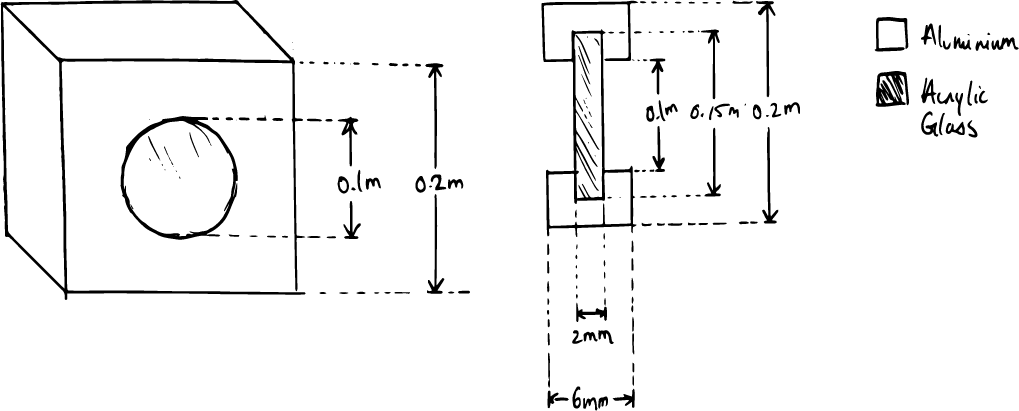
\includegraphics[width=0.85\linewidth]{fig/camera_custom_boitier_vect.png}
    \caption{Design du boîtier}
    \label{fig:boitier_camera_custom}
\end{figure}

\begin{table}[!htb]
\footnotesize
\centering
\scalebox{1.1}{
    \begin{tabular}{|c|c|c|c|c|c|}
    \hline
    \multirow{2}{*}{Concepts} & \multicolumn{4}{c}{Aspects de l'analyse} & \multirow{2}{*}{Décision} \\
    & Physiques & Économiques & Temporels & Socio-envir & \\
    \hline\hline
    GoPro Hero7 Black & Oui, mais & Oui & Oui & Oui & Retenue, mais\\
    HP2W Hyperfire 2 & Oui, mais & Oui & Oui & Oui & Retenue, mais \\
    GoFishCam & Oui & Oui & Oui & Oui & Retenue \\
    Capteur OV5640 & Oui, mais & Oui & Oui & Oui & Retenue, mais \\
    \hline
    \end{tabular}
}
\caption{Évaluation globale des concepts pour capter les informations sur les poissons}
\label{t:Decision_capteur}
\end{table}

\subsection{Alimenter le capteur}
 Cette fonction permet l'alimentation en énergie du système. C'est une fonction assez importante car le système a besoin d'énergie pour fonctionner. Le client demande un système capable de fonctionner 24 heures sur 24 pour une durée minimum de 14 jours en zone éloignée. Ainsi les aspects que nous utiliserons pour évaluer les critères de faisabilités sont les suivants : 
 \textbf{Aspects physiques:}
 \begin{itemize} [label = {--}]
    \item Dimensions de la solution et intensités
\end{itemize}
 \textbf{Aspects économiques:}
 \begin{itemize} [label = {--}]
    \item La solution doit être la moins coûteuse possible
\end{itemize}
 \textbf{Aspects temporels:}
 \begin{itemize} [label = {--}]
    \item Durabilité, c'est a dire un minimum de 14 jours
\end{itemize}
 \textbf{Aspects socio-environnementaux::}
 \begin{itemize} [label = {--}]
    \item Le système doit être sécuritaire pour l'environnement
\end{itemize}
 \subsubsection{Batterie au lithium :}
 \textbf{Description :}
 Pour alimenter notre systeme on peut se servir des batteries au lithium telle que  Energizer Ultimate Lithium. Ces piles, lorqu'elles sont utilisées dans certains capteurs comme la camera HP2X Hyperfire 2, ont une duree de vie s'etalant sur deux ans ou encore 40000 images ce qui nous permettra de repondre aux attentes du client. En plus d'une bonne durée de vie, les couts de ces bateries sont tres bas, on parle de 17.87 dollars la douzaine chez walmart. Performantes dans les temperatures extremes allant de -40 à 60 dégrés celsius, elles gardent leurs energies pendant 20 ans losqu'elles sont entreposées. Ces batteries de 1.5V chacune ne sont pas rechargeables et ne presentent pas de risques pour l'environnement.
 \textbf{Décision :}
 Retenue
 \textbf{Justification :}
 Avec une bonne durée de vie et peu couteuse, cette option respecte nos contraintes economiques et temporels. Aussi en empilant un certain nombre de ces batteries on aboutie a une alimentation fiable et securitaire, de ce fait nos contraintes physiques et socio-environnementaux sont egalement respectées.
 \subsubsection{Batterie au plomb :}
 \textbf{Description :}
 
 \textbf{Décision :}
 
 \textbf{Justification :}
 
 \subsubsection{Filaire:}
 \textbf{Description :}
 
 \textbf{Décision :}
 
 \textbf{Justification :}
 
 \subsubsection{Paneaux solaires:}
 \textbf{Description :}
  Le panneau solaire externe donne également une autre possibilité pour alimenter notre système. Il est muni d'un coffre de 8" * 8" qui contient une baterie rechargeable de 12V avec prise d'alimentation externe, qui est rechargée en permanence par le panneau solaire via un cable de 3'. Avec une puissance de 7 watts et des dimensions de 13" * 14", le panneau solaire est une option un peu plus dispendieuse , son prix est de 299.99 dollars (reconyx). Ce prix inclut tout le cablage ainsi que le materiel de montage. Les avantages de cette option c'est surtout la permanence de l'energie qui permettra a notre système de fontionner sans interruption.
 \textbf{Décision :}
 
 \textbf{Justification :}
 
 \begin{table}[!htb]
\footnotesize
\centering
\scalebox{1.2}{
    \begin{tabular}{|c|c|c|c|c|c|}
    \hline
    \multirow{2}{*}{Concepts} & \multicolumn{4}{c}{Aspects de l'analyse} & \multirow{2}{*}{Décision} \\
    & Physiques & Économiques & Temporels & Socio-envir & \\
    \hline\hline
    Batterie au lithium & Oui & Oui & Oui & Oui & Retenue\\
    Batterie au plomb & Oui & Oui & Oui & Oui & Retenue \\
    Filaire & Oui & Oui & Oui & Oui mais & Retenue mais \\
    Panneaux solaires & Oui & Non & Oui & Oui mais & Rejetée \\
    \hline
    \end{tabular}
}
\caption{Évaluation globale des concepts pour l'alimentation du système}
\label{t:Decision_alimenter}
\end{table}

\subsection{Acheminer les informations au centre de contrôle}
Cette composante se devra de transférer les données brutes de poissons, de température et de l'heure à un poste de contrôle pour les traiter et les compiler. Elle agit donc en tant que connexion entre le capteur et le poste de contrôle. Il est à considérer que le capteur peut se situer jusqu'à 15.25m sous l'eau et que les informations doivent être acheminées à une distance d'au moins 50m à travers l'eau. 


\subsection{Identifier les poissons et compiler les données}
Cette composante a pour fonction de transformer et compiler les données brutes recueillies par les différents capteurs pour créer les vignettes. Elle devra donc être en mesure d'identifier les espèces de poissons à partir des données du capteur. De plus, elle se chargera de comptabiliser le nombre de poissons de chaque d'espèces et de produire des statistiques.


\subsection{Stocker les données}
La composante qui occupera cette fonction devra enregistrer toutes les données pertinentes pour la base de données, c'est-à-dire les vignettes et les commentaires, les statistiques, les paramètres de configuration, les alarmes  qui ont été envoyées, les données de poissons de référence et les images originales prises par le capteur.
Comme mentionné à la section \ref{subsection:capacite_stockage}, ces données totaliseront un minimum de 200Go.

\textbf{Aspects physiques:}
\begin{itemize} [label = {--}]
    \item Le système soit pouvoir stocker au moins 200 Go de données.
\end{itemize}

\textbf{Aspects économiques:}
\begin{itemize} [label = {--}]
    \item La solution doit être la moins coûteuse possible
\end{itemize}

\textbf{Aspects temporel:}
\begin{itemize} [label = {--}]
    \item La conception de la solution doit respecter les délais alloués
\end{itemize}

\textbf{Aspects socio-environnementaux:}
\begin{itemize} [label = {--}]
    \item Les données stockées doivent être le plus facilement accessibles aux utilisateurs
\end{itemize}

\subsubsection{Carte mémoire SD SanDisk 32 Go classe 10 :}

\textbf{Description :} La carte mémoire SD SanDisk 32 Go classe 10 est une carte mémoire utilisée pour conserver les photographies en haute résolution utilisée sur les appareils photos compacts et de portée moyenne. Il a une capacité de stockage de 32 Go. Il peut stocker des vidéos en haute définition. La carte mémoire possède également une vitesse de transfert de 80 Mo/s. Également, il est dit que cette carte est étanche et résistante aux chocs et aux rayons X. Le système possède également une étiquette inscriptible lors de prise de photos et de vidéos. Elle coûte 13.98 dollars sur Amazon.

\textbf{Décision :} Rejetée.

\textbf{Justification :} Cette carte est très intéressante pour ce projet car elle est étanche, donc, résistante à l’eau et aux chocs et il serait également possible de récupérer les données même en cas de bris de la machine. La carte SD est très intéressante aussi pour sa vitesse de transferts. En effet, elle pourrait transférer ses informations à une vitesse très rapide pour la transmission d’une photographie. Enfin, grâce à l’étiquette inscriptible, il sera plus facile de concevoir la vignette. Cependant, on ne peut pas utiliser la carte SD car elle ne possède pas une capacité suffisante.

\textbf{Références :} \cite{casd} \cite{amsd}

\subsubsection{Cloud de hubiC}
\textbf{Description :} La plateforme Cloud de hubiC est un système informatique en nuage disponible sur la plateforme internet de Google. Un système d’informatique en nuage est un concept permettant d’enregistrer des données sur des ordinateurs localisés à distance grâce à une connexion en ligne et de pouvoir utiliser ces mêmes données à distance des ordinateurs. HubiC est une compagnie qui propose un service de stockage de données par nuage gratuitement jusqu’à 25 Go. Deux autres forfaits sont offert : 10 euros par an pour 100 Go et 50 euros par an pour 10 To. Pour assurer le transfert de données vers les serveurs de hubiC une connexion Internet est nécessaire puis il sera possible de suivre l’évolution des données à partir d’une grande diversité d’appareils (tablette, ordinateurs, téléphones intelligents…). 

\textbf{Décision :} Retenue.

\textbf{Justification :} Grâce à ce système nous pourrions facilement utiliser les données à partir d’un ordinateur. En effet, les données seront directement transmises par Internet, les photographies seraient transférées jusqu’à un ordinateur qui traitera alors les images. On choisit hubiC car il s’agit du système qui garantit gratuitement la plus grande capacité de données en nuage.  En acheminant l’information jusqu’au serveur, on pourra alors traiter les informations très rapidement. Pour 50 euros par an, on pourrait parfaitement sauvegarder toutes les données pendant 2 ans et on pourrait y accéder avec n’importe quel ordinateur.

\textbf{Références :} \cite{hubic} \cite{clgo} \cite{incl}

\subsubsection{Disque dur sur SSD Kingstone Digital SSD A400 SATA 3 }
\textbf{Description :} Un disque dur sur SSD (Solid State Drive) est un type de disque dur utilisant une mémoire électronique (en opposition aux disque dur mécaniques). Les disques durs représentent un intérêt pour plusieurs raisons : ils sont plus rapides, ils sont silencieux, ils consomment moins d’énergie et ils sont plus résistants aux chocs. Ainsi, cela permet de sauvegarder une quantité importante de données tout en étant très discret et autonome. Cependant, comme c’est un outil de sauvegarde de données fait à base d’électronique, on remarque une usure progressive du système. Le disque dur SSD Kingstone Digital SSD A400 SATA 3 proposé par Kingstone nous propose 240 Go de données disponible pour 39.99 dollars sur Amazon. 

\textbf{Décision :} Retenue.

\textbf{Justification :} Le disque dur SSD Kingstone Digital SSD A400 SATA 3 est un outil pratique pour sauvegarder beaucoup de données. En effet, 240 GB représentent une quantité de données disponible amplement suffisante pour le stockage des données sur la durée établie par le client. Le prix entre également amplement dans les frais matériel établie par le client. Malgré tout, même si l’usure affecte normalement les disques durs, ici, un seul client présente un mécontentement sérieux et ne concerne pas la durée de vie du disque dur.

\textbf{Références :} \cite{AMSSD} \cite{DESSD}

\subsubsection{Disque dur sur HDD Western Digital SATA III }

\textbf{Description :} Les disques durs HDD (Hard Disk Drive) sont des disques durs mécaniques servant à la sauvegarde des données. Ce sont des disques durs mécaniques où l’information est gravée sur des disques tournant à une grande vitesse. Ainsi, on peut accéder aux données gravées même après la fermeture de l’ordinateur qui traite les données. On remarque que les HDD sont moins coûteux que les SSD dans le ratio : données par dollars. Cependant, les HDD sont plus lents que les SSD. Celui proposé par Western Digital permet de stocker 1 To de données pour 54,99\$ sur Amazon. Il a une capacité de 200 000 photographies numériques et il a une garantie de deux ans. 

\textbf{Décision :} Retenue.

\textbf{Justification :} Ce disque dur a une capacité capable de stocker les informations que nous sauvegarderons sur la durée des deux ans. En effet, il peut sauvegarder jusqu’à 1 To. Également, même si elle est moins résistante, en théorie, que le disque dur SSD, il y a une garantie égale à la durée d’utilisation, voulue par le client, de la machine.

\textbf{Références :} \cite{HDD1} \cite{HDD2}

\begin{table}[!htb]
\footnotesize
\centering
\scalebox{1.2}{
    \begin{tabular}{|c|c|c|c|c|c|}
    \hline
    \multirow{2}{*}{Concepts} & \multicolumn{4}{c}{Aspects de l'analyse} & \multirow{2}{*}{Décision} \\
    & Physiques & Économiques & Temporels & Socio-envir & \\
    \hline\hline
    Carte SD & Non & Oui & Oui & Oui & Rejetée\\
    Cloud & Oui & Oui & Oui & Oui & Retenue \\
    Disque dur SSD & Oui & Oui & Oui & Oui & Retenue \\
    Disque Dur HDD & Oui & Oui & Oui & Oui & Retenue \\
    \hline
    \end{tabular}
}
\caption{Évaluation globales des concepts pour le stockage de données}
\label{t:Decision_stockage}
\end{table}



\subsection{Afficher les données}
Cette composante devra afficher les données d'une manière efficace et conviviale pour les employés du MFA. Cette interface assurera la communication avec l'utilisateur pour visualiser les données et configurer les différents paramètres. \vspace{5mm}

\textbf{Aspects physiques:}
\begin{itemize} [label = {--}]
    \item N/A
\end{itemize}

\textbf{Aspects économiques:}
\begin{itemize} [label = {--}]
    \item La solution doit satisfaire un excellent rapport qualité/prix
\end{itemize}

\textbf{Aspects temporel:}
\begin{itemize} [label = {--}]
    \item La conception de la solution doit respecter les délais alloués
\end{itemize}

\textbf{Aspects socio-environnementaux:}
\begin{itemize} [label = {--}]
    \item La solution doit présenter les données de manière efficace et conviviale
\end{itemize}


\subsubsection{Application web avec Ajax}

\textbf{Description:} Ajax est une série de techniques de développement web qui utilise une combinaison de langage tel que JavaScript, XML, HTML et CSS pour créer des applications web. La page web performe automatiquement un appel JavaScript à l'engin Ajax, ce qui correspond à une requête XMLHttpRequest. Puis, une requête HTTP est envoyé au serveur afin de retrouver la donnée appropriée. Cette donnée est ensuite retourner à Ajax sous forme HTML, XML ou Javascript pour être livrée à la page web.  \vspace{5mm}
% Reste à trouver les coûts


\textbf{Décision:} Retenue. \vspace{5mm}

\textbf{Justification:} L'avantage d'Ajax est qu'il crée des applications web dites asynchrones. Ainsi, les applications web peuvent envoyer et retourner des données d'un serveur sans affecter l'affichage de la page web courante. Les requêtes au serveur se font sans attendre la demande de l'utilisateur, ce qui optimise la performance de l'interface. En d'autres mots, le contenu de la page peut changer dynamiquement sans que l'utilisateur ait besoin de rafraîchir la page. De cette manière, il serait possible de voir en temps réels les données des population de poissons. \vspace{5mm}
% J'ai pas finis

\textbf{Références:} \cite{Ajax_wiki} \cite{Ajax}

\subsubsection{Application web et mobile avec PrimeFaces}

\textbf{Description:} PrimeFaces offre plusieurs modèles d'application web à l'aide de serveur Java. Ces modèles comprennent également l'interaction avec plusieurs autres appareil, comme les tablettes et les téléphones intelligents. PrimeFaces permet ainsi la création d'application web et mobile. Par exemple, le modèle Roma 

\textbf{Décision:} Retenue.

\textbf{Justification:} PrimeFaces comprends une variété de modèles d'application web de haute qualité. Les prix des licences complètes varient entre 320\$ et 1050\$ dépendamment du modèle choisis. L'utilisation de PrimeFaces est efficace et robuste. Elle promet une expérience client facile d'utilisation.

\textbf{Références:} \cite{PF} \cite{PF_Roma} \cite{PF_exemple}


\subsection{Assurer un accès sécurisé}
Cette fonction est présente dans le but de garder les données confidentielles et de limiter le contrôle du capteur seulement aux utilisateurs autorisés. % Il faudra donc déterminer une méthode d'identification.

\begin{table}[htp]
   \footnotesize
   \centering
   \scalebox{1}{
   \begin{tabular}{|c|c|c|c|}
        \hline
        Section 1 & Section 2 [unités] & ... & ... \\
        \hline\hline
        Texte & Encore texte & ... & ... \\
        Texte & Encore texte & ... & ... \\
        Texte & Encore texte & ... & ... \\
        Texte & Encore texte & ... & ... \\
        \hline
   \end{tabular}}
\caption{Accès sécurisé}
\label{t:securite}
\end{table}


\subsection{Mesurer la date et l'heure}

\subsection{Mesurer la température externe} 
Tel que voulu par le client, notre capteur doit être capable de mesurer la température de l’eau, c’est-à-dire la température de l’environnement à l’extérieur du capteur. Il est importé de mesurer cette température car le ministère a précisé que le capteur devait fonctionner dans des températures de l’eau allant de -4 °C jusqu’à 25 °C. Ainsi, on doit être capable de transférer l’information de la température de l’eau dans la vignette. La température influe sur le milieu de vie des poissons et il est important de savoir si la température n’atteint pas un point critique, un point à partir duquel le capteur pourrait rencontrer un disfonctionnement. 

\textbf{Aspects physiques:}
\begin{itemize}[label = {--}]
    \item Sous l'eau, la solution doit posséder une masse inférieure à 5kg
    \item Sous l'eau, la solution doit posséder un volume de moins de 0.3m$^3$
    \item La solution doit être utilisable jusqu'à une profondeur de 50 pieds
    \item La température interne de la solution doit être entre +5°C et -10°C par rapport à la température de l'eau
    \item La température de l'eau doit être entre -4 °C et 25 °C
    \item La solution doit être opérationnelle en tout temps pendant une période de 14 jours au minimum
    \item La solution doit être fonctionnelle sur une durée d'au moins 2 ans
\end{itemize}

\textbf{Aspects économiques:}
\begin{itemize}[label = {--}]
    \item La solution doit être la moins dispendieuse possible
\end{itemize}

\textbf{Aspects temporels:}
\begin{itemize}[label = {--}]
    \item Le temps de développement de la solution doit être minimisé
\end{itemize}

\textbf{Aspects socio-environnementaux:}
\begin{itemize}[label = {--}]
    \item La solution doit assurer une mesure passive
\end{itemize}

\subsubsection{Thermomètre de cuisson intelligent d’Accu-Temp :}
\label{subsubsection:accu-temp}

\textbf{Description:} Le Thermomètre de cuisson intelligent d’Accu-Temp est un thermomètre d’abord conçu pour la cuisson dans un four par la compagnie Accu-temp, une entreprise spécialisée dans l’équipement commercial de cuisine. De ce fait, ce thermomètre est conçu pour résister à des températures extrêmes. Ainsi, il est admis qu’il peut résister à des températures allant de -25 à 300 degrés Celsius. Également, le but de ce thermomètre est de prévenir l’utilisateur lorsque le temps de cuisson est élevé et il est possible d’y voir la température. Pour mieux utiliser ce thermomètre de cuisson, il est compatible avec une application disponible gratuitement permettant de voir le temps de cuisson ainsi que la température et le moment. Le prix le moins cher est celui de 49,99 dollars canadiens (avant taxes).\vspace{5mm}

\textbf{Références}: \cite{Ares} \cite{AmAc} \cite{CaAc} \vspace{5mm}

\textbf{Décision}: Retenue mais

\textbf{Justification}: Cet outil de cuisine correspond aux contraintes établies et atteint les objectifs voulus. En effet, dans un premier temps, il reste fonctionnel dans l’écart de température établie par le client. Théoriquement, ce thermomètre intelligent serait capable de transmettre ses informations jusqu’à une distance de 30 mètres par Bluetooth à partir d’un four en action. Cependant, en se fiant sur les différents commentaires sur le site de Canadian Tire, on voit que certains des consommateurs qui se sont procuré le thermomètre affichent leur mécontentement. Un des points soulevés est son inaptitude réelle à transmettre l’information par Bluetooth. En effet, un de ces consommateurs écrit qu’en réalité, le thermomètre ne pouvait en réalité ne fonctionner qu’à une portée maximale de 5 mètres en pratique. De ce fait, on peut se demander si on peut réellement faire confiance au thermomètre concernant ce critère. De plus, ce thermomètre nécessitant une alimentation par piles, sa durée de vie semble être limitée.

Exemple: on a déjà présenté ce concept au point \ref{subsubsection:accu-temp} et les mêmes critères s'appliquent.

\subsubsection{Thermistance NTCLE100E3103JT2 placée à l’extérieur reliée à un Arduino Uno:}
\label{thermis}

\textbf{Description :} Une thermistance est un outil résistif au courant qui varie en fonction de la température environnante. La NTCLE100E3103JT2 est une de ces thermistances de la gamme NTCLE100E3possédant une zone d’efficacité allant de -40 à 125 °C et atteignant une valeur de 10 000 ohms à 25 °C. On peut se procurer cette thermistance pour 1.21 dollars sur Digikey. Un Arduino Uno est un microcontrôleur conçu par Arduino pouvant être utilisé comme ampèremètre et pouvant transmettre ses informations via un câble USB. De ce fait, grâce à la loi d’Ohm, on sait que U=R*I et on peut grâce au microcontrôleur programmer une fonction capable de transformer la valeur du courant en valeur de la température puis de transmettre ces informations à une commande centrale via le câble USB. Ce microcontrôleur coûte 20.69 dollars sur amazon. 

\textbf{Références :} \cite{TuAr} \cite{DaTh} \cite{AmAr}

\textbf{Décision :} Retenue

\textbf{Justification :} Grâce à un circuit rudimentaire et un code simple, ce concept pourrait tout à fait remplir sa fonction. En effet, ce circuit n’est composé que de deux éléments. En mesurant le courant grâce à l’Arduino, on tire l’expression mathématique liée à la résistance en fonction de la température de la thermistance. Étant donné que l’Arduino peut fournir une source de tension continue, il est très simple d’exprimer la température en fonction du courant. Ces transformations seront effectuées à l’aide d’un code dans l’Arduino (l’Arduino pouvant déjà être utilisé comme voltmètre, on n’a plus qu’à établir des équations mathématiques simples). Enfin, ces données pourront être transmises grâce à l’Arduino et de son câble USB. Il faut également penser à ne placer que la partie de la thermistance dans l'eau sans que le reste du circuit y touche, sinon, il pourrait y avoir des problèmes en cas de submersion.

\subsubsection{Thermomètre intelligent Thermo de Withings:}

\textbf{Description :} Le thermomètre intelligent Thermo de Withings est un thermomètre médical utilisé pour mesurer par le toucher les parois d’un être humain. Il s’agit d’un thermomètre intelligent capable, grâce à une application mobile, d’informer l’utilisateur de la température actuelle et mesurer à chaque fois. Il prévient des moments opportuns pour prendre certains médicaments spécifiques pour soigner. Il est précis à 0.2 °C près. Il nécessite une connexion Wi-Fi. Il peut également conserver les données de plusieurs cibles simultanément. Il atteint un coût de 99,95 dollars américains.

\textbf{Références :} \cite{Thermo}

\textbf{Décision :} Rejetée

\textbf{Justification :} Ce thermomètre est conçu pour mesurer des parois humaines. Donc, il doit être capable de mesurer des températures situées autour de 37 °C. De ce fait, comme aucunes mesures de températures extrêmes ne sont marquées, on ne peut pas affirmer qu’il sera capable de mesurer des températures allant de -4 à 25 °C. De plus, ce concept est beaucoup plus coûteux que les autres proposés précédemment. Pour cette raison, nous ne pouvons pas nous permettre de présenter ce concept au client. 

\subsubsection{Diode 1n4148 avec un Arduino Uno : }
\label{1n4}

\textbf{ Description :}La diode 1n4148 est un semi-conducteur fait à partir de silicone. LE but premier d’une diode est d’assurer le passage du courant lorsque la différence de potentielle dépasse la tension de seuil et que le courant circule dans le même sens que ce semi-conducteur. Une des caractéristiques de la diode 1n4148 est le fait que la tension entre l’anode et la cathode diminue lorsque la température augmente. On observe alors un ratio de 2,2 millivolts par °C. À partir de cette information, on peut établir un rapport pour la mesure de la température ambiante autour de la diode. Cela est rendu possible grâce à un microcontrôleur de type Arduino Uno, présenté précédemment. Il faut payer 0.018 dollars pour un paquet de 10 sur alliedelec.com. La diode reste efficace entre -30 et 120 °C.

\textbf{Références :} \cite{Allie} \cite{Tu1n}  \cite{Da1n}

\textbf{Décision :} Retenue

\textbf{Justification :} Tel que vu avec la thermistance, on peut utiliser un Arduino Uno avec une programmation simple et un circuit simple afin de parvenir à mesurer la température ambiante. De surcroît, le circuit reste fonctionnel dans l’écart de température établit par le client. Il faut toutefois considérer le fait que seulement la diode doit toucher l'eau.

\begin{table}[!htb]
\footnotesize
\centering
\scalebox{0.9}{
    \begin{tabular}{|c|c|c|c|c|c|}
    \hline
    \multirow{2}{*}{Concepts} & \multicolumn{4}{c}{Aspects de l'analyse} & \multirow{2}{*}{Décision} \\
    & Physiques & Économiques & Temporels & Socio-envir & \\
    \hline\hline
    Thermomètre d'Accu-Temp & Oui mais  & Oui & Oui mais & Oui & Retenue mais \\
    Thermistance & Oui & Oui & Oui & Oui & Retenue \\
    Thermo de Withings & Non & Oui mais & Oui & Oui & Rejetée \\
    Diode 1n4148 avec un Arduino Uno & Oui & Oui & Oui & Oui & Retenue \\
    \hline
    \end{tabular}
}
\caption{Évaluation globales des concepts pour la mesure de la température externe}
\label{t:Decision_thermo_ext}
\end{table}


\subsection{Mesurer la température interne}
Le capteur est essentiellement construit de composantes électroniques. Ainsi, à des températures extrêmes, il pourrait rencontrer des dysfonctionnements si jamais le capteur atteignait des températures capables de s'attaquer aux composantes électroniques. De ce fait, le client a exigé que le capteur ait une température intérieure entre -10°C et 5°C au delà de la température de l'eau. Ainsi, à des cas extrêmes, le capteur doit posséder une température entre -14°C et 30°C.

\textbf{Aspects physiques:}
\begin{itemize}[label = {--}]
    \item Sous l'eau, la solution doit posséder une masse inférieure à 5kg
    \item Sous l'eau, la solution doit posséder un volume de moins de 0.3m$^3$
    \item La solution doit être utilisable jusqu'à une profondeur de 50 pieds
    \item La température interne de la solution doit être entre +5°C et -10°C par rapport à la température de l'eau
    \item La température à l'intérieur du capteur doit être entre -14°C et 30°C.
    \item La solution doit être opérationnelle en tout temps pendant une période de 14 jours au minimum
    \item La solution doit être fonctionnelle sur une durée d'au moins 2 ans
\end{itemize}

\textbf{Aspects économiques:}
\begin{itemize}[label = {--}]
    \item La solution doit être la moins dispendieuse possible
\end{itemize}

\textbf{Aspects temporels:}
\begin{itemize}[label = {--}]
    \item Le temps de développement de la solution doit être minimisé
\end{itemize}

\textbf{Aspects socio-environnementaux:}
\begin{itemize}[label = {--}]
    \item La solution doit assurer une mesure passive
\end{itemize}

\subsubsection{HP2W Hyperfire 2 Professionnal White Flash Camera}
\textbf{Description :} Cet élément a déjà été présenté au point \ref{subsubsectionHyperfire}

\textbf{Références :} \ref{subsubsectionHyperfire}

\textbf{Décision :} Retenue

\textbf{Justification :} Certes, l'outil est dispendieux et prend de l'espace. Cependant, considérant qu'il peut être utilisé comme capteur pour les photographies, on pourrait économiser, car tout en prenant les photographies, on pourrait avoir la température intérieure du capteur. Ainsi, on le retient car malgré son coût et son volume, il peut remplir plusieurs tâches simultanément.

\subsubsection{Thermomètre au mercure H-B instrument 2/1110 Durac}
\textbf{Description :} Un thermomètre au mercure est un outil de mesure de la température. Lorsque la température monte, le mercure prend l'expension jusqu'à indiquer la température mesurée. Celui-ci coûte 24,96 \$ sur Amazon. Il a une incertitude de 2°C et peut mesurer des températures allant de -20 °C jusqu'à 110°C.

\textbf{Références :} \cite{mercure}

\textbf{Décision :} Rejetée

\textbf{Justification :} Certes, ce thermomètre a la capacité de mesurer la température estimée du capteur. Cependant, cet outil n'étant aucunement relié à un outil numérique, il faudrait trouver un moyen de transmettre l'information détenue par le thermomètre jusqu'à la vignette. Ainsi, il faudrait surveiller constamment la température inscrite par le thermomètre afin de savoir la température du capteur, une opération qui peut s'avérer très complexes. Ainsi, on ne choisira pas cette option afin de mesurer la température interne du capteur.

\subsubsection{Diode 1n4148 avec un Arduino Uno :}
\textbf{Description :} Ce concept a déjà été présenté au point \ref{1n4}

\textbf{Référence :} \ref{1n4}

\textbf{Décision :} Retenue

\textbf{Justification :} Tel qu'expliqué précédemment, on pourra facilement mesurer la température dans l'écart de température voulu et transmettre les informations facilement pour un prix réduit. Ainsi cette option sera considérée. 

\subsubsection{Thermistance NTCLE100E3103JT2 placée à l’extérieur reliée à un Arduino Uno :}
\textbf{Description :} Le concept a déjà été présenté au point \ref{thermis}

\textbf{Références :} \ref{thermis}

\textbf{Décision :} Retenue

\textbf{Justification :} Comme on l'a vu auparavant, on pourrait facilement mesurer la température interne du capteur avec ce système et transférer les informations pour la vignette. L'écart de température toléré couvre celui désiré par le client. Cette option est donc gardée.

\begin{table}[!htb]
\footnotesize
\centering
\scalebox{0.9}{
    \begin{tabular}{|c|c|c|c|c|c|}
    \hline
    \multirow{2}{*}{Concepts} & \multicolumn{4}{c}{Aspects de l'analyse} & \multirow{2}{*}{Décision} \\
    & Physiques & Économiques & Temporels & Socio-envir & \\
    \hline\hline
    Camera Hyperfire & Oui  & Oui & Oui & Oui & Retenue \\
    Thermomètre au mercure & Non & Oui & Oui & Oui & Rejetée \\
    Thermistance & Oui & Oui mais & Oui & Oui & Retenue \\
    Diode 1n4148 avec un Arduino Uno & Oui & Oui & Oui & Oui & Retenue \\
    \hline
    \end{tabular}
}
\end{table}


\subsection{Analyser l'état du système}
Cette fonction traitera si une alarme doit être générée. Il y aura une alarme lorsque le fonctionnement du système pourrait être compromis, c'est-à-dire si il y la température interne excède l'intervalle de résistance à la température des composantes du capteur, si l'identification est impossible sur plusieurs captures ou si il y a une brèche de sécurité.
